\documentclass{article}
\usepackage{geometry}
 \geometry{
 a4paper,
 total={170mm,257mm},
 left=20mm,
 top=20mm,
 }
\usepackage{graphicx}
\usepackage{hyperref}
\usepackage{biblatex}
\usepackage{amsmath,amssymb}
\usepackage{subcaption}

\addbibresource{sources.bib}

\author{Meftah, Morteza M.D; Waren, Daniel M.D; Bosco, Joseph A. IV;\\
Di Gangi, Catherine; Watson, Cody Ph.D}
\title{Modeling Robotic Surgery Predictions: Write-Up}

\begin{document}

\maketitle

\textbf{%
DISCLAIMER:
This is a VERY rough draft of the write-up. 
It is meant to demonstrate the work I have done on the project in a way that you don't need to read any code.
Document written by Jack Bosco. 
Code for the data analysis, modeling, and visualization are also written by Jack Bosco. 
}

\section{Introduction}

Coronal Plane Alignment of the Knee (CPAK) morphologies are powerful visualization tools for pre-operative planning in Total Knee Replacement (TKA) cases. \cite{MacDessi2021-mi}
Dispite this useful metric, there exists no method for to predicting the optimal post-resection alignment based on the pre-operative alignment.
In this study, we propose the NYU model to predict optimal post-operative aHKA alignement 
for achieving suitable laxity during a total knee replacement based on the pre-operative aHKA value.

\subsection{Background}

Classification of knee alignment into CPAK morphologies consists of two measurements: the Joint Line Obliquity (JLO) and the anterior Hip Knee Alignment (aHKA).
Anterior Hip Knee Alignment (aHKA) is the angle between the femoral and tibial mechanical axes in the coronal plane.
Joint Line Obliquity (JLO) is the angle between the femoral and tibial mechanical axes in the sagittal plane.
Sections of the CPAK classification allow physicians to envision the alignment of the hip and knee in a 3D space \cite{MacDessi2021-mi}.

\subsection{Motivation} % Can we find a predictive model for implant alignment based on pre-operative deformity

The motivation for this project is to find a predictive model for implant alignment based on pre-operative deformity.
When in the planning phase for a total knee arthroplasty (TKA), the surgeon must predict the femoral resection amounts 
(Medial Distal, Lateral Distal, Medial Posterior, Lateral Posterior)
and the tibial resection amounts 
(Medial, Lateral)
most likely to yeild suitable laxity for the implant.

These predictions may be informed by the pre-operative deformity of the knee.
As aHKA values differ from the mean, alignments are Varus or Valgus according to the following rule ($\alpha=2$):

\[\text{lateral morphology}=
	\begin{cases}
		\text{Varus} & \text{if } \text{aHKA} < -\alpha \\
		\text{Valgus} & \text{if } \text{aHKA} > \alpha \\
		\text{Aligned} & \text{if } \text{aHKA} \in [-\alpha, \alpha]
	\end{cases} ^ \text{\cite{MacDessi2021-mi}}
\]

Dispite the usefulness of this metric, there exists no method for to predicting the optimal post-resection alignment based on the pre-operative alignment.
In this study, we propose the NYU model to predict optimal post-operative aHKA alignement 
for achieving suitable laxity during a total knee replacement based on the pre-operative aHKA value.

\section{Methods}

Analysis of pre-operative planning and report screenings from 626 TKR cases was used to build a predictive model
to approximate optimal post-resection aHKA value based on the pre-operative aHKA value.
Consecutive records were collected from hospital records and agregated by the senior author into a single dataset.
The dataset was then cleaned and pre-processed to remove any missing or incomplete data, yeilding 626 complete cases in total (Figure \ref{fig:cpak_ref}).

\begin{figure}[ht]
	\caption{Data Visualization and Clustering}
	\begin{subfigure}[lt]{.4\textwidth}
		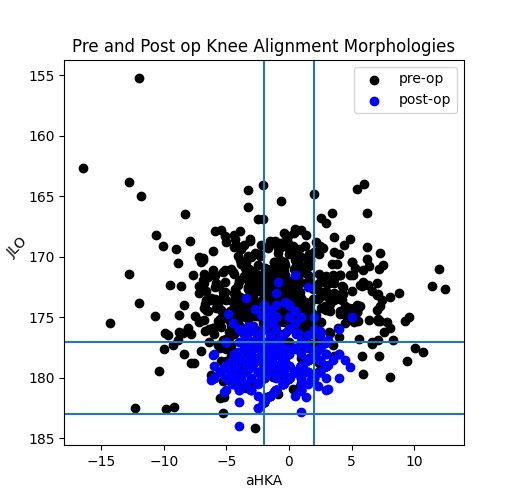
\includegraphics[width=\linewidth]{data_vis.png}
		\caption{%
			\footnotesize
			These are the averages of the clusters - See CPAK reference.\\
			Top: Pre and post-op data displayed on a scatterchart of Joint Line Obliquity (JLO) and anterior Hip Knee Alignment (aHKA)\\
			Bottom: Average Pre and post-op alignment grouped by pre-operative aHKA values.\\
			The average change from pre-op to post-op is shown.
			}
		\label{fig:cpak_ref}
	\end{subfigure}
	\begin{subfigure}[rt]{.58\textwidth}
		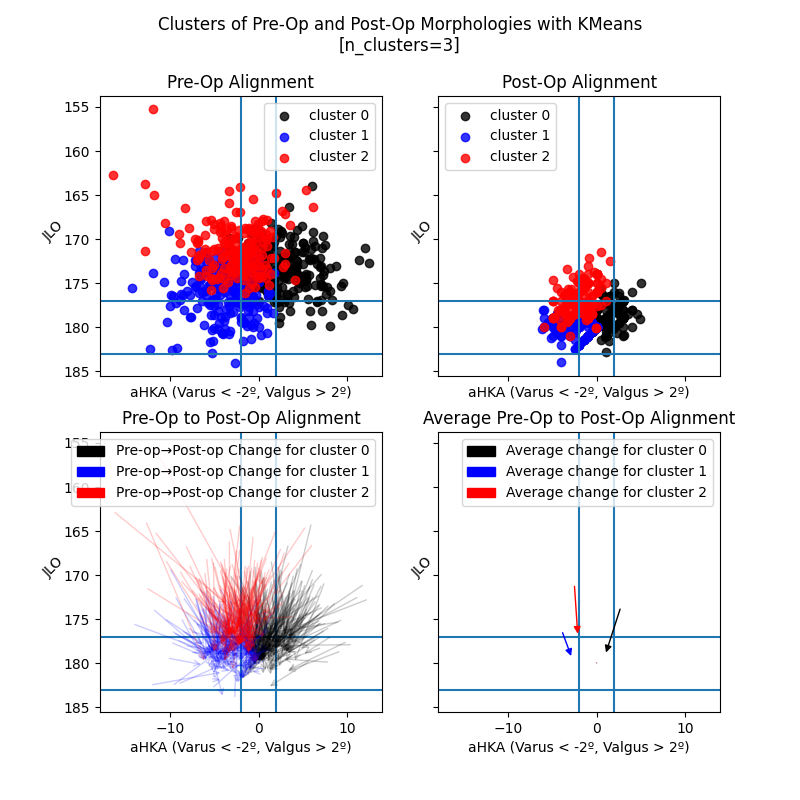
\includegraphics[width=\linewidth]{clusters.png}
		\caption{%
			\footnotesize
			Bottom Left: Arrows are drawn for each pre and post-operative pair (one pair per case).\\
			Bottom Right: Averages are taken for each cluser and the change from pre-op to post-op is shown.
			}
		\label{fig:clusters}
	\end{subfigure}
\end{figure}



For the analysis, the pre-operative aHKA values were standardized using either the standard scaler method or min-max scaler method.
Then, the pre-operative alignments were clustered using the K-means clustering algorithm
(see \href{https://scikit-learn.org/stable/modules/generated/sklearn.cluster.KMeans.html#sklearn.cluster.KMeans}
{\underline{Sklearn K-Means Clustering}}) (Figure \ref{fig:clusters}.)\\

\section{Results} % list what I looked at and what the results were

Several models were trained to predict the optimal post-resection aHKA value based on the pre-operative aHKA value:
\begin{itemize}
	\item A linear regression model (Figure \ref{fig:degree_3_polynomial_regression})
	\item A support vector machine model (Figure \ref{fig:svm_regression})
	\item A multi-layer perceptron model (Figure \ref{fig:neural_network_regression})
\end{itemize}

\begin{figure}[ht]
	\caption{Regression Models}
	\begin{subfigure}{.32\textwidth}
		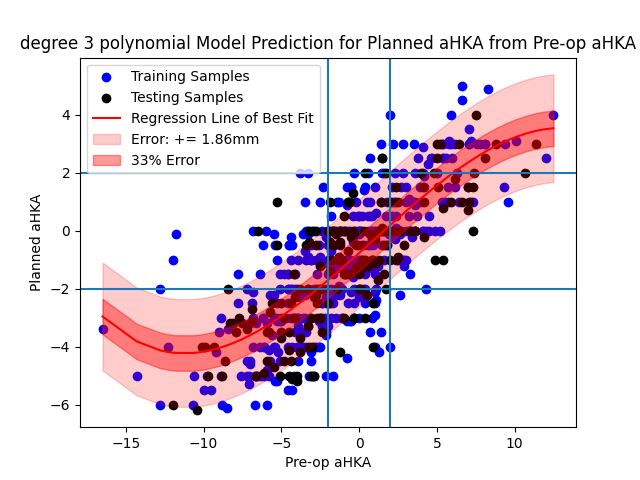
\includegraphics[width=\textwidth]{degree_3_polynomial_regression.png}
		\caption{}
		\label{fig:degree_3_polynomial_regression}
	\end{subfigure}
	\begin{subfigure}{.32\textwidth}
		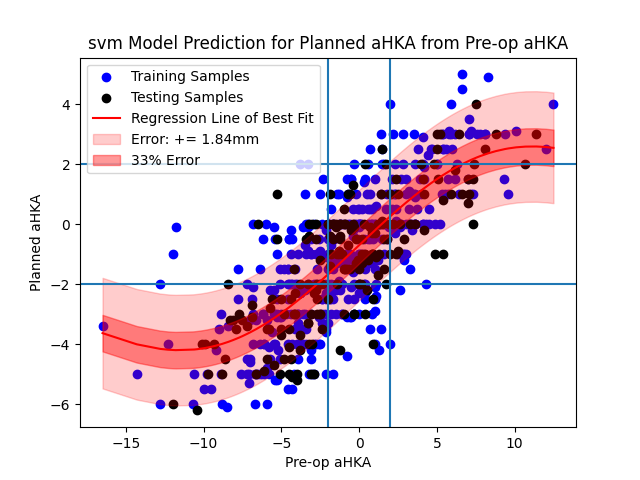
\includegraphics[width=\textwidth]{svm_regression.png}
		\caption{}
		\label{fig:svm_regression}
	\end{subfigure}
	\begin{subfigure}{.32\textwidth}
		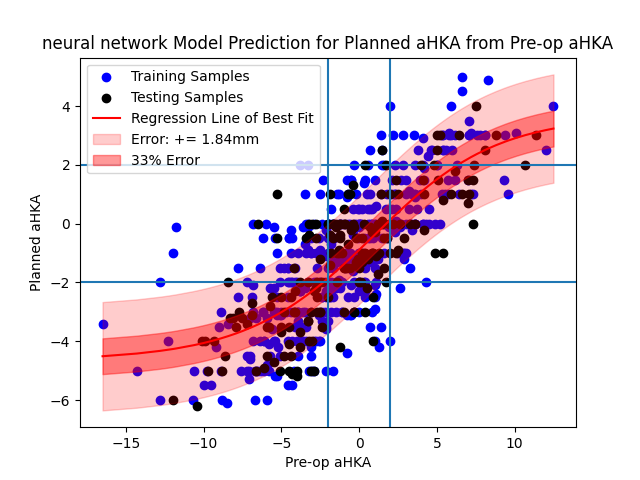
\includegraphics[width=\textwidth]{neural_network_regression.png}
		\caption{}
		\label{fig:neural_network_regression}
	\end{subfigure}
	\caption*{
		\footnotesize
		Regression models trained using Polynomial, SVM, and Neural Network regression training algorithms, respectively.
		The error is the mean squared distance from the testing set (black).
		The regression is trained on the training set (blue)
	}
	\label{fig:regression_models}
\end{figure}

To train the polynomail regression model \ref{fig:degree_3_polynomial_regression}, input features are transformed using a polynomial transformation of degree 3 
(see \href{https://scikit-learn.org/stable/modules/generated/sklearn.linear_model.LinearRegression.html}{\underline{Sklearn Polynomial Features}}).
Afterwards, the model is trained using a linear regression algorithm 
(see \href{https://scikit-learn.org/stable/modules/generated/sklearn.linear_model.LinearRegression.html}{\underline{Sklearn Linear Regression}}).

For the support vector regressor \ref{fig:neural_network_regression} the pre and post-operative aHKA values were standardized using the standard scaler method.
Then, the model is trained using a nu support vector regression algorithm
(see \href{https://scikit-learn.org/stable/modules/generated/sklearn.svm.NuSVR.html#sklearn.svm.NuSVR}{\underline{Sklearn Support Vector Machine}}).

For the deep learning model \ref{fig:svm_regression} pre and post-operative aHKA values were normalized using the min-max scaler method with feature range $[-1, 1]$ in the pretraining step.
Then, the model is trained using a multi-layer perceptron (MLP) algorithm 
(see \href{https://scikit-learn.org/stable/modules/generated/sklearn.neural_network.MLPRegressor.html}{\underline{Sklearn Multi-layer Perceptrion}}).

\medskip

\printbibliography

\end{document}

